\chapter{Background}\label{cha:chapter3}

\section{Neural Networks}
Neural networks(NNs) are a type of machine learning algorithms that try to mimic how human brain works.  In particular, NNs have units called neurons connecting together similar to the way neurons in our brain do. These connections allow NNs to build hierarchical representations that are necessary to perform an objective task. \addfigure{\ref{fig:nn_simple}} illustrates a simple reaction task that neurons in our brain perform together to achieve.

 \begin{figure}[ht!]
    \begin{center}

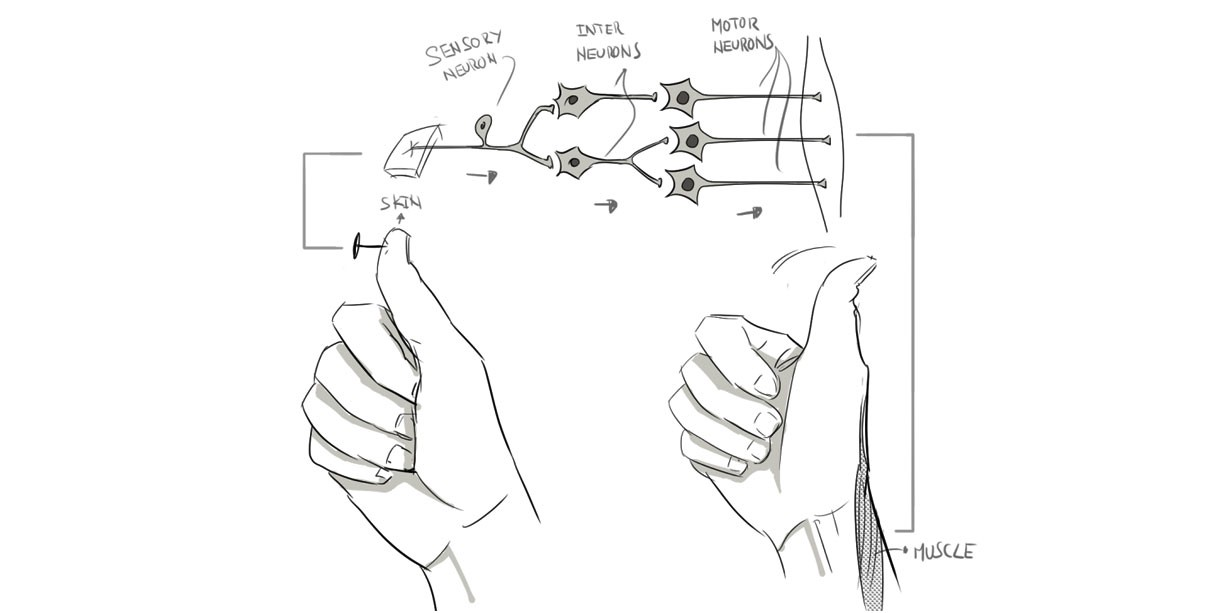
\includegraphics[width=\textwidth]{nn_simple}
\caption{An illustration of how neurons in human brain cooperate together to sense the pain and react accordingly.}
\small{Source : \cite{LeonMakingSimpleNeural2017}}
\label{fig:nn_simple}

\end{center}
\end{figure}

 \begin{figure}[ht!]
    \begin{center}

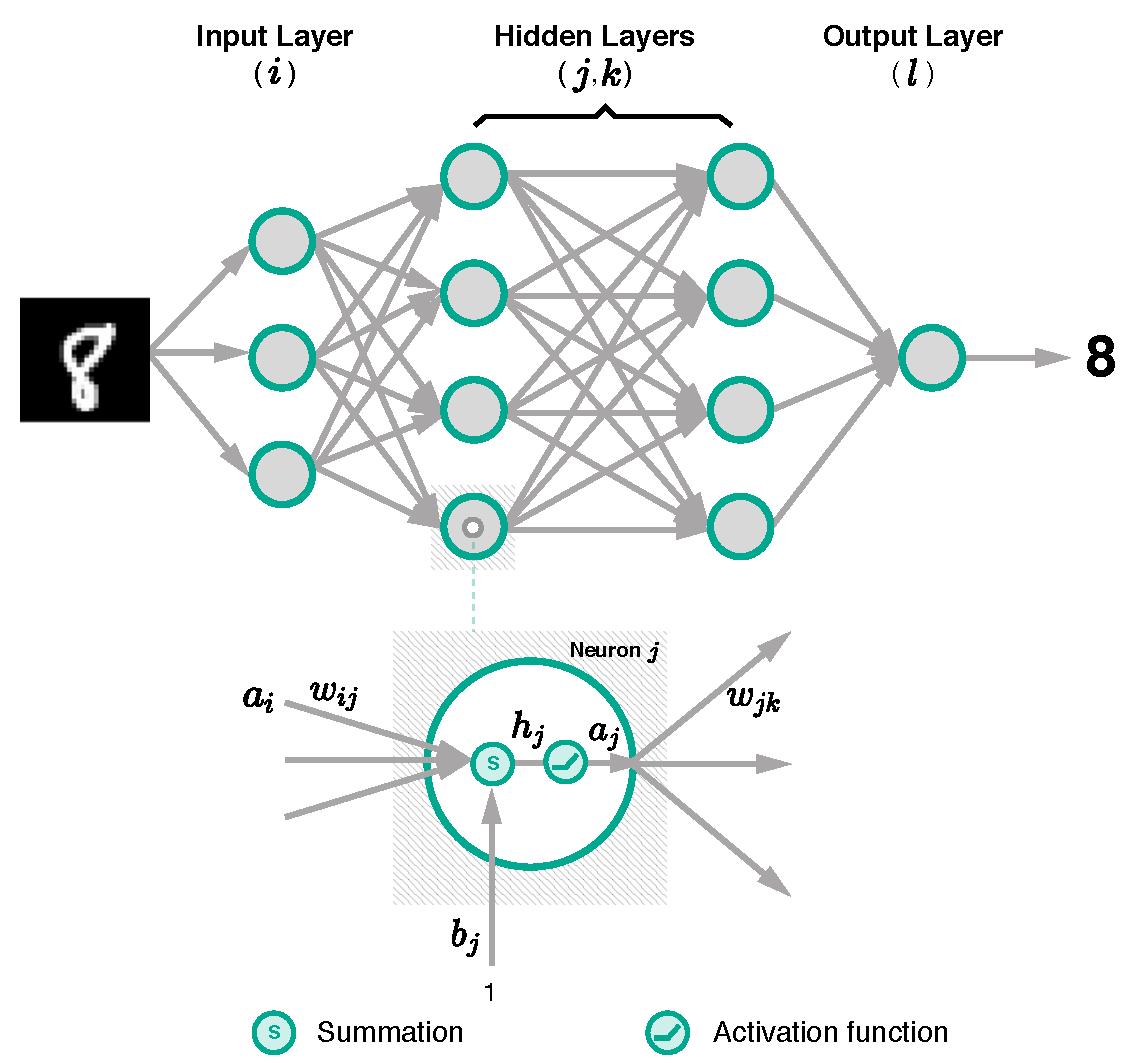
\includegraphics[width=0.8\textwidth]{sketch/typical_nn_structure}
\caption[]{A general structure of neural networks and details of a neuron's connectivity and activity.}
\label{fig:nn_typical_structure}

\end{center}
\end{figure}


% \begin{figure}[ht!]
%	\begin{center}
%
%		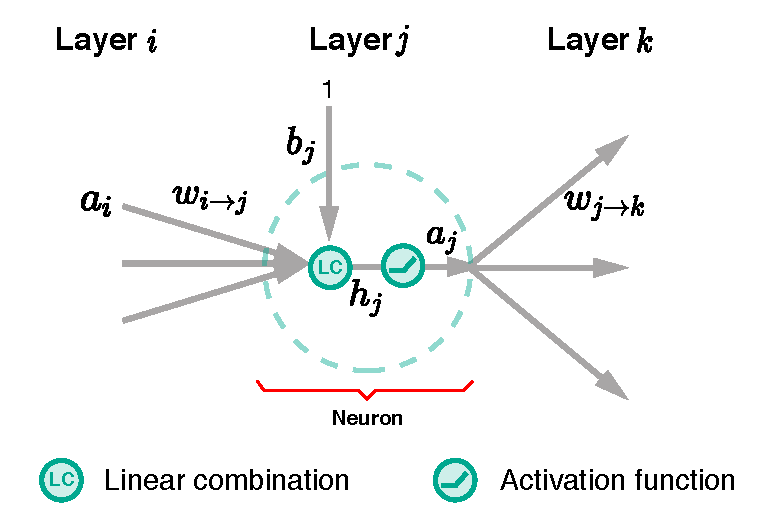
\includegraphics[width=0.5\textwidth]{sketch/a_neuron}
%		\caption{Connectivity and activity of a neuron}
%		\label{fig:a_neuron}
%	\end{center}
%\end{figure}


\addfigure{\ref{fig:nn_typical_structure}} illustrates a general structure of NNs. The network has input layer, output layer and hidden layers, which are analogous to sensory, motor and inter neurons in \addfigure{\ref{fig:nn_simple}}. The figure also shows connections of a neuron to other neurons in previous and later layer. Given an objective task, the goal is to construct connections between these neurons such that the network can transform input into a desired output.  This connections are determined by trainable variables, called weights and biases. They are denoted by $w_{i\rightarrow j}, w_{j\rightarrow k}$ and $b_j$ respectively in the figure, and will be learned  in during \textit{training} process.  In this example, the objective task to classify what is the given digit.


Consider a given set of $p$ training samples $\mathcal{D} = \{ \xa, \ya) \}_{\alpha=1}^{p}$,  there are 3 primary components to train a NN, namely  
\begin{enumerate}
	\item \textbf{Network architecture} defines the configuration of NN. Some of important settings are number of layers and number of neuron in each layer and type of activation function. These settings determine neurons' activity and how they communicate to each other through connections governed by trainable weights and biases. Typically, the weights and biases are denoted as $\patvector{\theta}$. Mathematically, NN can be viewed as a function $f$ with parameters $\patvector{\theta}$ that nonlinearly transforms an input $\xa\in \mathbb{R}^d $ to some output.
	\item \textbf{Loss function $L$}  is a measurement corresponding to the objective task. It quantifies how far output $f(\xa)$ from the NN far the true output $\ya$. If we average the loss over some samples,  we call the result as \textit{Cost} and denote it as $J$.
	\item \textbf{Learning algorithm} is responsible for optimizing trainable variables in the network such that the overall loss is minimized. Practically, we learn this variables through optimizing the cost of training samples \textit{Empirical Error}. This is a proxy to optimize the cost of the data distribution(\textit{Generalization Error}). 
\end{enumerate}

Hence, the goal of this empirical training process can be summarized as follows : 

\begin{align} \label{eq:nn_opt}
	\patvector{\hat{\theta}} = \patarg{min}{\theta} \underbrace{\frac{1}{p}  \sum_{\alpha=1}^p L( f(\xa), \ya) }_{J}
\end{align}

\subsection{Loss functions}
Choosing loss function is depend on the objective that the network is being trained to solve. For classification problems, such as digit classification, whose goal is to categorize $\x$ into a category $C$ from $K$ categories, $f : \x \in \mathbb{R}^d  \mapsto C \in \{ C_k \}_{k=1}^K$, \textit{Cross-Entropy}(CE) is the loss function for this purpose.
$$
L_{\text{CE}} = - \sum_{i} y_k \log \hat{y}_k,
$$
where $y_i \in [0, 1]$ and $\hat{y}_i \in [0, 1]$ are true and predicted probability that $\x$ belongs to $C_k$ respectively. Denote $\patvector{z} = f(\x) \in \mathbb{R}^{K}$. $\hat{y}_k$ is computed via \textit{softmax} function :
$$
\hat{y}_k = \frac{e^{z_k}}{ \sum_{k=1}^K{e^{z_k}} }
$$ 

For regression problems, $ f : \x \in \mathbb{R}^d  \mapsto \mathbb{R}$, such as price forecast,\textit{Mean Squared Error}(MSE) is the loss function.
$$
L_{\text{MSE}} = (f(\x) - y)^2
$$

This is a brief introduction to loss functions widely used in machine learning. More loss functions do exist and are beyond scope of the thesis to cover.

\subsection{Learning Algorithm : Gradient Descent and Backpropagation}
Due to substantial number of trainable variables in a neural network, it is crucial to solve the optimization (\ref{eq:nn_opt}) efficiently. The answer to solve this high dimensional problem is to use repeated procedure, called \textit{Gradient Descent}.  \addfigure{\ref{fig:gradent_descent_toy}} provides an intuition of the method. Consider a  function $J(\theta)$ on the figure as a toy example of a cost function of a NN with a parameter $\theta$. The figure shows that if we gradually adjust $\theta$ in the opposite direction of gradient, $	-\frac{d L(\theta)}{d \theta}$,  with a proper step size $\lambda$ (\textit{learning rate}), we will eventually reach one of the minimals. This update  is summarized in (\ref{eq:gradient_update}).


% In this case, $\hat{\theta}$ can trivially computed by solving
%
%\begin{align}
%	\frac{d L(\theta)}{d \theta}  \stackrel{!}{=} 0
%	\label{eq:simple_solve_for_thetha}
%\end{align}

\begin{figure}[!hbt]
    \begin{center}
		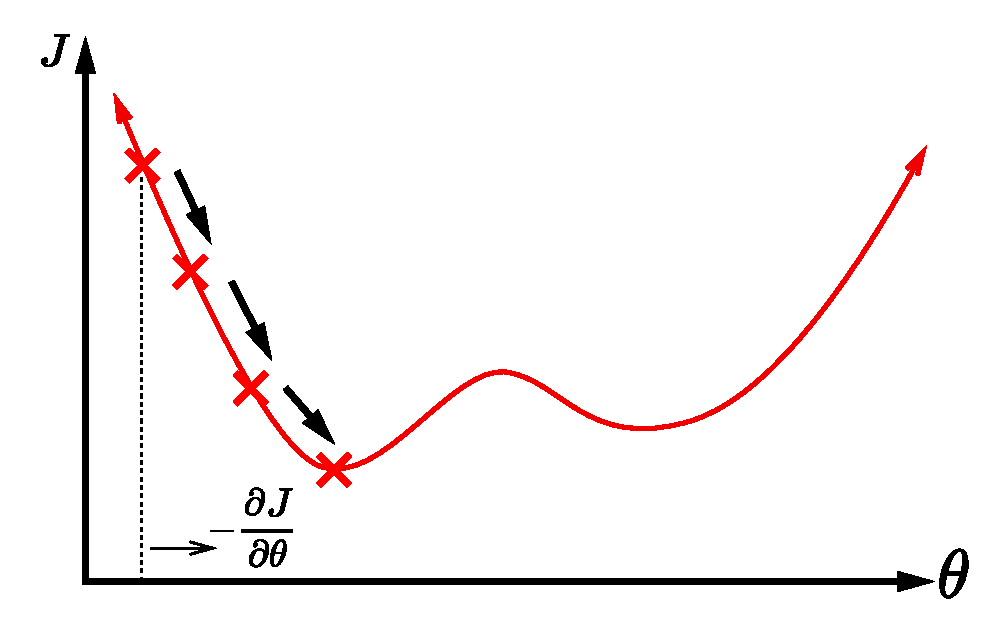
\includegraphics[width=0.6\textwidth]{sketch/gradient_intuition}
		\caption[]{An illustration of Gradient Descent}
		\label{fig:gradent_descent_toy}
	\end{center}
\end{figure}

\begin{align}
 \theta_i \leftarrow \theta_i - \lambda  \frac{\partial J }{\partial \theta_i}, \forall \theta_i \in \btheta
\label{eq:gradient_update}
\end{align}


Let's consider again the NN shown in \addfigure{\ref{fig:nn_typical_structure}}. Assume that the network uses an activation function $\sigma$ and has $\btheta = \{ \forall i,j,k,l : w^{(1)}_{i \rightarrow j}, w^{(2)}_{j \rightarrow k}, w^{(3)}_{k \rightarrow l}  \}$ with biases omitted. For a sample $(\xa, \ya)$, $f(\xa )$ is  calculated as follows

\begin{align*}
		h_j^{(1)} &= \sum_i w_{i \rightarrow j}^{(1)} x_i^{(\alpha)} & a_j^{(1)} &= \sigma (h_j^{(1)})	\\
		h_k^{(2)} &= \sum_j w_{j \rightarrow k}^{(2)} a_j^{(1)}  & a_k^{(2)} &= \sigma (h_k^{(2)})	 \\
		h_l^{(3)} &= \sum_k w_{k \rightarrow l}^{(3)} a_k^{(2)} & a_l^{(3)} &= \sigma (h_l^{(3)})	 \\
		f(\x) &= [ a_1^{(3)}, \dots, a_L^{(3)}  ]^T  & J &= \frac{1}{p} \sum_{\alpha = 1}^{p} L(f(\xa), \ya)	
\end{align*}

The gradients can be then computed by recursively applying chain rule from the last to the first layer, hence the name \textit{Backpropagation}.
\begin{align}
	\frac{\partial l(f(\xa), \ya)  }{\partial w_{k \rightarrow l}^{(3)} } &= 	\frac{\partial l(f(\xa), \ya) }{\partial a_{l}^{(3)} }  \frac{\partial a_{l}^{(3)} }{\partial w_{k \rightarrow l}^{(3)} }  	\\
		&= 	\underbrace{\frac{\partial l(f(\xa), \ya) }{\partial a_{l}^{(3)} } \sigma'(h_l^{(3)})}_{ \delta_l^{(3)}} a_{k}^{(2)} 	\\
	\frac{\partial l(f(\xa), \ya)  }{\partial w_{j \rightarrow k}^{(2)} } 
		&=  \sum_{l' = 1}^{L} 	\frac{\partial l(f(\xa), \ya) }{\partial a_{l'}^{(3)} } \frac{\partial a_{l'}^{(3)}}{\partial w_{j \rightarrow k}^{(2)}} \\
		&= \sum_{l' = 1}^{L} 	\frac{\partial l(f(\xa), \ya) }{\partial a_{l'}^{(3)} } \sigma'(h_{l'}^{(3)})  \frac{\partial h_{l'}^{(3)} }{\partial w_{j \rightarrow k}^{(2)}} \\
		&= \sum_{l' = 1}^{L} 	\delta_{l'}^{(3)}  w_{k \rightarrow l'}^{(3)} \frac{\partial a_{k}^{(2)} }{\partial w_{j \rightarrow k}^{(2)}} \\
		&= a_{j}^{(1)}  \underbrace{\sigma'(h_{k}^{(2)}) \sum_{l' = 1}^{L} 	\delta_{l'}^{(3)} w_{k \rightarrow l'}^{(3)}}_{\delta_{k}^{(2)}}  \\
	\frac{\partial l(f(\xa), \ya)  }{\partial w_{i \rightarrow j}^{(1)} } &=  x_i  \sigma'(h_{j}^{(1)}) \sum_{k' = 1}^{K} 	\delta_{k'}^{(2)} w_{j \rightarrow k'}^{(2)} 
\end{align}
As shown in the derivations above, \textit{Backpropagation} allows us to efficiently compute the gradients by reusing calculated gradients from the later layer, for example $\delta_l^{(3)}, 	\delta_{k}^{(2)}$. Moreover, $\delta_l^{(3)}, 	\delta_{k}^{(2)}$ can also interpreted as error propagated to responsible neurons.

In practice, because the training set usually contains several thousand samples, the gradient update in  (\ref{eq:gradient_update}) would require significant amount of computation to update just one step, not to mention that it could also result in small gradient update step leading to slow convergence to desire objective performance. Therefore, the training data $D$ is usually divided into batches  $\widetilde{D}_i$  with equal size and perform the gradient update for every $\widetilde{D}_i$. For example, the size of $\widetilde{D}_i$ is usually chosen between 32 and 512 samples. This refers to \textit{Mini-Batch Gradient Descent}.

Lastly, because noise in training data and potentially highly non-smooth of the cost function, learning rate $\lambda$ has great influential on the training process. More precisely, it should not be too small or too large. This requires some effort and experience in order to get the right value. Some work have proposed alternative update rules aiming to make the training process more stable. For example,  Adaptive Moment Estimation(Adam)\cite{KingmaAdamMethodStochastic2014}  uses adaptive learning rate  and incorporates accumulated direction and speed of the previous gradients(\textit{momentum}) into the update, hence more consistent gradient and fast convergence. Other similar proposals are RMSProp \cite{TielemanLectureRmsPropDivide2012} and Adadelta \cite{ZeilerADADELTAAdaptiveLearning2012}.


\subsection{Convolutional Neural Networks} \label{sec:conv}
Convolutional Neural Networks(CNNs) refer to neural networks that employ convolutional operators to process information in early layers instead of fully-connected layers(weighted sum). Typically, a convolutional operator is followed by a pooling operator. Using this convolutional and pooling operators allows the neural network to extract hierarchical features that are spatially invariant \cite{ZeilerVisualizingUnderstandingConvolutional2013}, hence leading to higher predictive capability comparing to traditional fully-connected layers with fewer number of parameters.

%\afterpage{
\begin{figure}[!hbt]
    \begin{center}
		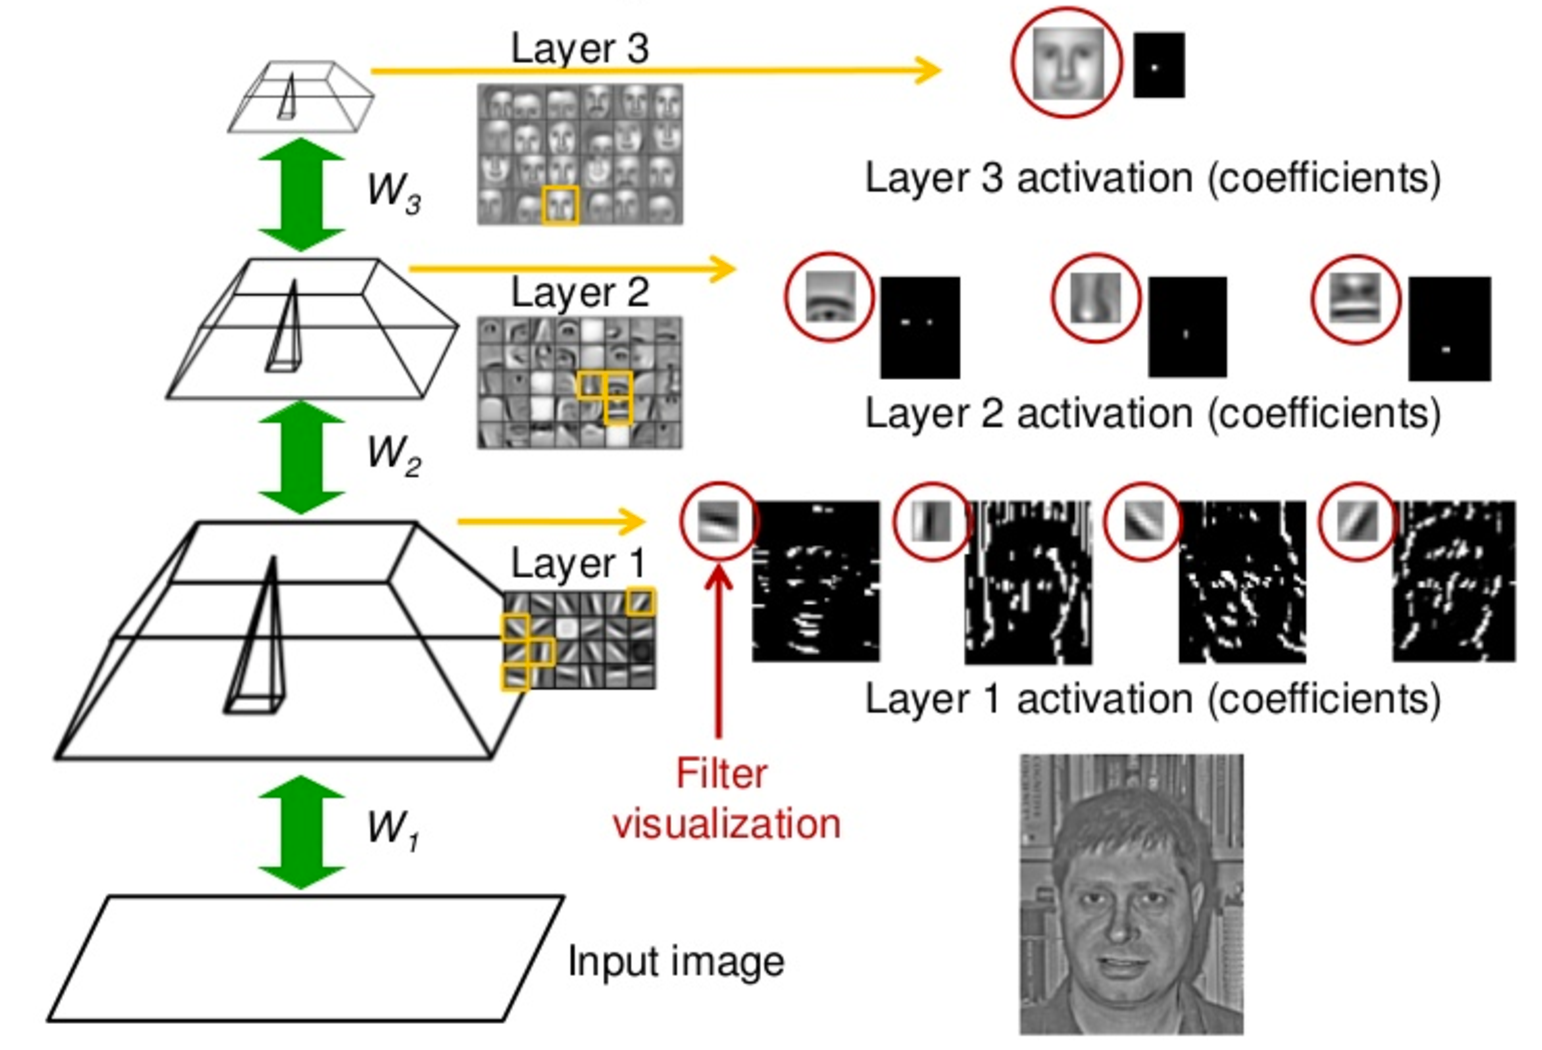
\includegraphics[width=0.5\textwidth]{sketch/cnn_hierachical_features}
		\caption{Hierarchical features learned by a CNN.}
		\label{fig:conv_intuition}
		\small{Source : \cite{LeeConvolutionalDeepBelief2009}}
	\end{center}
\end{figure}


\addfigure{\ref{fig:conv_intuition}} illustrates hierarchical structures that neurons in each layer of a CNN learn to detect. More precisely, this example shows that neurons in the first learn to detect low level features, such as edges, and neurons in middle layer then use knowledge to detect higher level features, for example nose, mouth or eyes, and so on.


%\afterpage{
\begin{figure}[!hbt]
    \begin{center}
		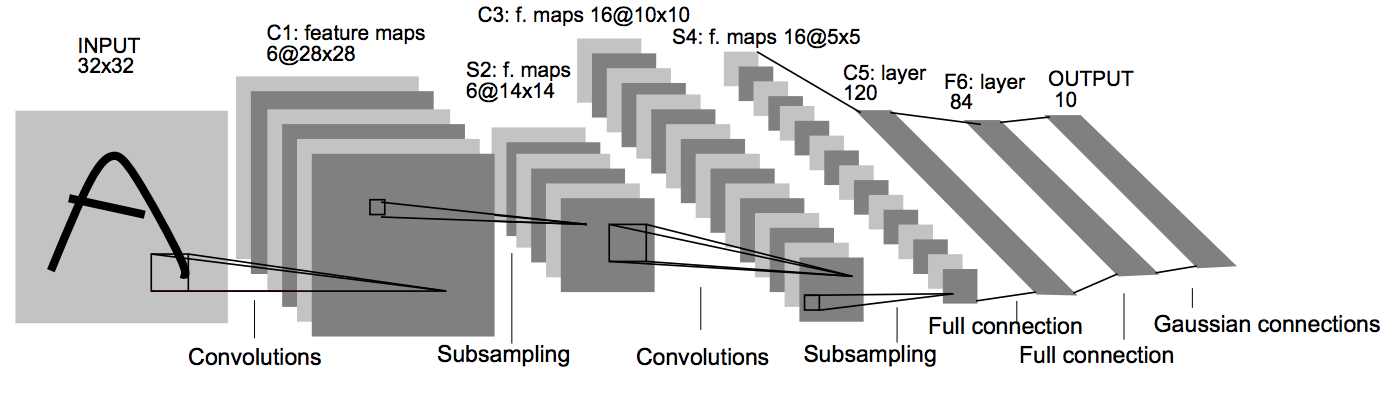
\includegraphics[width=0.8\textwidth]{lenet}
		\caption{LeNet-5 architecture for a digits recognition task.}
		\label{fig:lenet}
		\small{ Source : \cite{LeCunGradientBasedLearningApplied2001} }
	\end{center}
\end{figure}


Since \cite{LeCunGradientBasedLearningApplied2001} proposed LeNet-5, shown in \addfigure{\ref{fig:lenet}}, and successfully applied it to handwritten recognition problems, CNNs have become the first choice of architectures in many domains. Particularly, in computer vision, CNNs are the core component of state-of-the-art results in various contests. Such successful results are :  AlexNet\cite{KrizhevskyImageNetClassificationDeep2012} that archive the remarkable results on  ImageNet Large-Scale Visual Recognition Challenge 2012(ILSVRC 2012) followed by the achievement of VGG\cite{SimonyanVeryDeepConvolutional2014} and GoogleLenet \cite{SzegedyGoingDeeperConvolutions2014} architecture in ILSVRC 2014 and ResNet\cite{HeDeepResidualLearning2015} that won ILSVRC 2015.



\subsection{Recurrent Neural Networks}
Recurrent Neural Networks(RNNs) are neural networks whose computed outputs   are repeatedly incorporated into its next computation. \addfigure{\ref{fig:rnn_unfold}} illustrates this idea of recurrent computation by unfolding RNN into steps. Let's consider $\x$ a sequence of $x_1, \dots, x_T$.  At step $t$, RNN takes $r_{t-1}$ and $x_{t}$ to compute $r_{t}$ and $\hat{y}_t$. This recurrent connections can be interpreted as accumulating information from the past, hence RNNs are well capable of processing sequential data, possibly  coming with different and not limited in length . Natural Language Processing(NLP) and Machine Translation(MT) are some of the fields that RNNs are widely applied to.


\begin{figure}[!hbt]
\centering
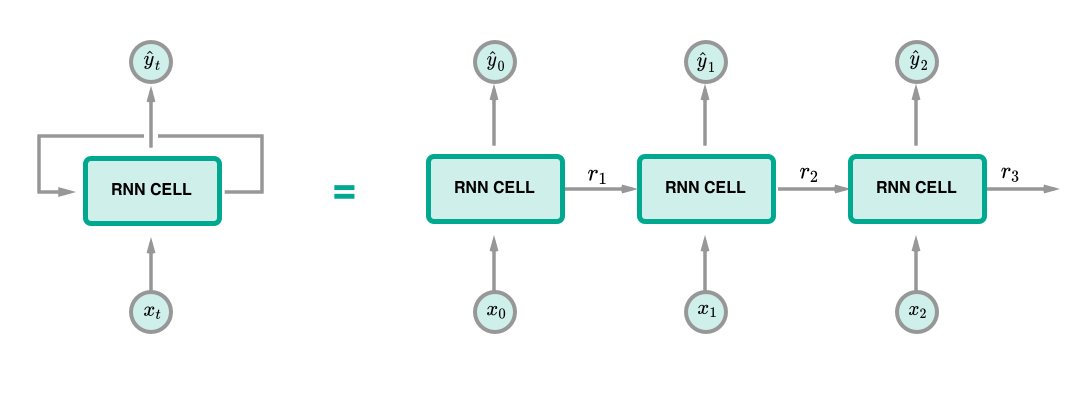
\includegraphics[width=0.8\textwidth]{sketch/rnn_unfold}
\caption{Unfolded RNN Structure}
\small{Inspired by a figure in \cite{OlahUnderstandingLSTMNetworks2015} }
\label{fig:rnn_unfold} 
\end{figure}


\subsubsection{Backpropagation Through Time}
As the number of computation steps in RNNs is depend on the length of samples, which can be different in principle, one needs to organize data in such a way that samples in the same batch have the same steps of computations before training a RNN. As a result, training RNNs can be viewed as training a feedforward neural network with a certain depth of layers, where we can then apply backpropagation. The difference from regular feedforward setting is that  variables are shared across layers.

Consider again the RNN in \addfigure{\ref{fig:rnn_unfold}} with $\x = \{x_1, \dots, x_T \}$ and $r_0 = 0$. Assume that only $\hat{y}_T$ determines the value of the loss function and the computations are defined as follows 
\begin{align}
	h_1 &= w_{rx} x_1 + w_{rr} r_0 & r_1 &= \sigma(h_1) \label{eq:naive_r} \\
	h_2 &= w_{rx} x_2 + w_{rr} r_1 &  r_2 &= \sigma(h_2) \\
	& \vdots & \vdots \\
	h_{T-1} &= w_{rx} x_{T-1} + w_{rr} r_{T-2} &  r_{T-1} &= \sigma(h_{T-1}) \\
	\hat{y} &= \sigma(w_{yx} x_T   + w_{yr} r_{T-1})
\end{align}

The gradients can be computed by 
\begin{align}
	\frac{\partial l}{\partial w_{yx}} &= \sigma'(w_{yx} x_T   + w_{yr} r_{T-1}) x_T \\
	\frac{\partial l}{\partial w_{yr}} &= \sigma'(w_{yx} x_T   + w_{yr} r_{T-1}) r_{T-1} \\
	\frac{\partial l}{\partial w_{rx}} &= 	w_{yr} \sigma'(w_{yx} x_T   + w_{yr} r_{T-1}) \frac{\partial r_{T-1}}{\partial w_{rx}} \\
	&= w_{yr} \sigma'(w_{yx} x_T   + w_{yr} r_{T-1})  \Bigg[ \sigma'(h_{T-1}) \bigg( x_{T-1} + w_{rr}  \frac{\partial r_{T-2}}{\partial w_{rx}} \bigg) \Bigg]  \label{eq:gradient_wrr}  \\
	\frac{\partial l}{\partial w_{rr}} &= w_{yr} \sigma'(w_{yx} x_T   + w_{yr} r_{T-1})  \frac{\partial r_{T-1}}{\partial w_{rr}}  \\
	&= w_{yr} \sigma'(w_{yx} x_T   + w_{yr} r_{T-1})  \Bigg[ \sigma'(h_{T-1}) \bigg( \frac{\partial r_{T-2}}{\partial w_{rr}} \bigg) \Bigg] \\
\end{align}
However, as we unfold the computations, we can see that there are 2 problems that might happen to the gradients of the shared parameters $w_{rx}$ and $ w_{rr}$, namely
\begin{itemize}
	\item Exploding Gradient : this scenario happens if the gradient is derived from shared weights, for example $w_{rr}$ in  (\ref{eq:gradient_wrr}), whose absolute value is greater than one. The recursive multiplication will result in a large value of the gradient leading to unreliable training. \cite{PascanuUnderstandingexplodinggradient2012} have proposed Gradient Clipping to alleviate the problem.
	\item Varnishing Gradient : in contrast, when the values are smaller than one, the gradient will be very small causing slow learning. More precisely, RNNs would require enormous of time to learn long term dependencies. The next section discusses techniques to mitigate this problem.
\end{itemize}


\subsubsection{Long Short-Term Memory and Gated RNNs}
Varnishing Gradient is a major problem that causes RNNs to learn long term memories with slow progress. This is due to the computation of recurrent connections are constructed. In particular, as in (\ref{eq:naive_r}), standard RNNs compute those connections with weighted sum at every step $t$ leading to recursive multiplication terms in the gradient's computation.

Alternatively, \cite{HochreiterLongshorttermmemory1997} have proposed \textit{Long Short-Term Memory}(LSTM) network that employs a gating mechanism and additive updates in the calculation of the recurrent connections. This mechanism decreases number of damping factors involved in the gradients' computation, hence it allows the network to learn long memories better.

As shown in \addfigure{\ref{fig:lstm_structure}}, LSTM utilizes 3 gates, namely input $i_g$, forget $f_g$ and $o_g$ output gate, to control the information flow through the LSTM cell. More precisely, $i_g$ and $f_g$ decides how to accumulate information from the previous cell state $C_{t-1}$, and an input cell state computed from previous output $h_{t-1}$ and current input $x_t$, into in the new cell state $C_t$. On the other hand, $o_g$ determines to control leakage of information from $C_t$ to outside $h_t$. Formally, 
\begin{align}
	i_g &= \sigma( w_{ix} x_t + w_{ih} h_{t-1} )  &  	f_g &= \sigma( w_{fx} x_t + w_{fh} h_{t-1} )\\
	o_g &= \sigma( w_{ox} x_t + w_{oh} h_{t-1} ) & \widetilde{C}_t &= \tanh(w_{cx} x_t + w_{ch} h_t) \\
	C_t &= f_g \otimes C_{t-1} + i_g  \otimes  \widetilde{C}_t & h_{t} &= o_g \otimes \tanh(C_t)
\end{align}


\begin{figure}[h]
\centering
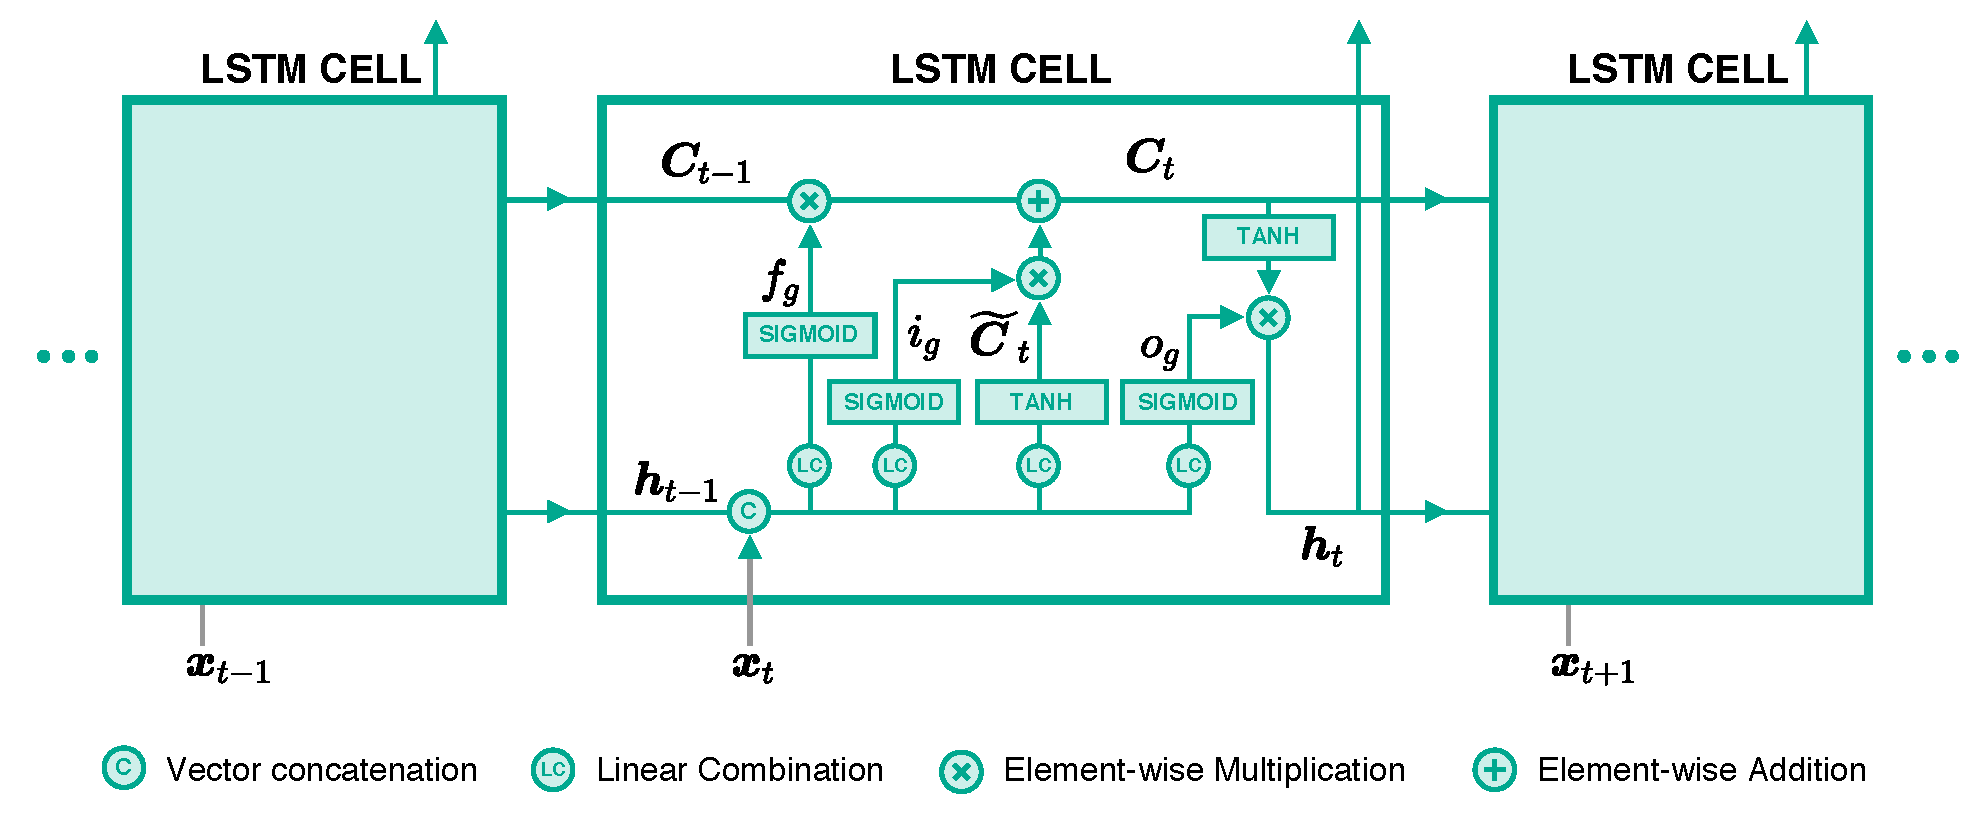
\includegraphics[width=1\textwidth]{sketch/lstm}
\caption{LSTM Structure} 

\label{fig:lstm_structure} 
\end{figure}

Since the work was published, LSTM has successfully contributed to many state-of-the-art results in Machine Translation(MT) and Natural Language Processing(NLP)\cite{MelisStateArtEvaluation2018}. \cite{GreffLSTMsearchspace2017} have shown that the forget and output gate are the crucial parts of the network.  \cite{ChoLearningPhraseRepresentations2014a} have proposed \textit{Gated Recurrent Unit}(GRU) that employs only 2 gates, however \cite{Jozefowiczempiricalexplorationrecurrent2015a} have conducted several benchmarking tasks and found no significant difference in performance between LSTM and GRU. 